\documentclass[12pt]{article}
\usepackage[margin=1.5cm]{geometry}
\usepackage{parskip}
\usepackage{amsmath}
\usepackage{amssymb}
\usepackage{amsfonts}
\usepackage{enumitem}
\usepackage{graphicx}
\usepackage{stmaryrd}
\graphicspath{ {./images/} }


\begin{document}
\begin{enumerate}[label=(\alph*)]

  \item
    \begin{enumerate}[label=(\roman*)]
      \item

        In this question, we assume that the routing protocol is using poison reverse, or else we get count-to-infinity.

        Assuming that $B$ and $C$ do not quickly respond to failure, there will be no path from $A$ to $C$.

        At the next iteration, both $B$ and $C$ will notice that their link is broken,  so assuming fewest-nodes is the tiebreaker metric, $B$ will transmit to $A$ that it can reach $C$ with a latency of 12ms through $E$, and will advertise to $E$ that it can reach $C$ with a latency of infinity through $E$. Similarly, $C$ will advertise to $D$ that it can reach $B$ with a latency of infinity through $D$.

        At the next iteration, $D$ tells $E$ that it has a route to $B$ with latency infinity, through $E$. At this point, $A$ and $E$ still believe they have a route to $B$ through $C$, since the news from $D$ has not travelled far enough yet.

        At the next iteration, $E$ now knows that the route to $B$ through $C$ no longer exists, so instead advertises to $A$ that it has a route to $B$ with length 8 (directly to $B$). $A$ still thinks that it can get to $B$ through $C$, so it does not advertise anything.

        Finally, $A$ recomputes the routes and learns that the best route to $B$ is directly to $B$, since the route through $E$ is now longer, and we reach a steady state, after around 2 minutes of waiting.

        After 5 minutes, the link is repaired.

        Since we are only concerned about routes to $B$, we will ignore routing messages from $B$, since for routing to $B$ they remain the same. $C$ advertises to $D$ that it has a route of distance 1 directly to $B$.

        On the next iteration, $D$ advertises this route to $E$.

        Finally, on the next iteration, $E$ advertises this route to $A$, and it is better than the route directly to $B$, so $A$ returns to the better route and we reach a steady state.

        This takes around 1 minute and 30 seconds of waiting.

      \item

        A graph is shown below:

        \begin{minipage}{\textwidth}
          \centering
          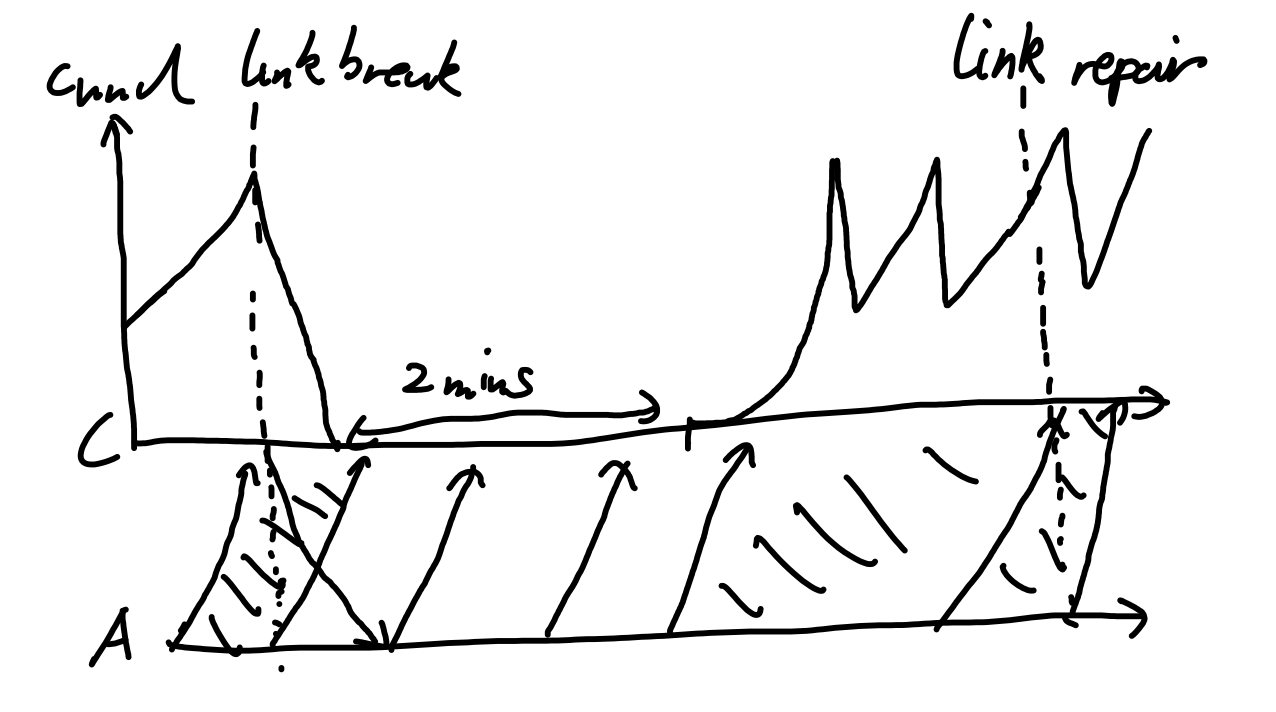
\includegraphics[scale=0.3]{time}
        \end{minipage}
    \end{enumerate}

  \item
    If we use link state routing, $A$ would have been immediately informed that the link from $B$ to $C$ was broken (as would all other nodes), and could have immediately recomputed the optimal path directly to $B$ instead. So, the TCP connection would only have failed for the time it took $B$ to inform $A$, as opposed to 2 minutes.

    Upon repair, $A$ would also have been immediately informed that the link from $B$ to $C$ was repaired by $B$, so could have immediately recomputed the optimal path back through $E$ instead. These routing computations might potentially have been more complicated, in the sense we have to run something like Dijkstra's algorithm locally at each node, but the complexity of the overall routing state is much simpler.

        
\end{enumerate}
\end{document}
